\section{Chromatin}

  %% Note that the size of an human genome is for an haploid genome.  The
  %% actual number of bp inside a typical cell will be double of that.
  %% Also, the estimate ignores mitochondrial DNA but at this scale its size
  %% is negligible anyway, and we are talking about fitting it into the
  %% nucleus anyway.
  The human genome has a length of some \num{3.2e9}
  base pairs \citep{nature-first-human-genome-draft}
  meaning that a diploid human cell will
  typically have \SI{6.4}{\giga\bp} of genomic information inside
  its nucleus.
  All of this is organised in a large DNA--protein complex known as chromatin.

  Access to the genomic information is not uniform in chromatin.
  It is organised in a hierarchical structure with
  multiple levels of compaction \frefp{fig:intro:chromatin-structure} where
  the level of compaction increases as access to the underlying genomic
  information decreases.
  This is often simplistically distinguished as
  euchromatin and heterochromatin for low and
  high compaction respectively, although more detailed categories of
  chromatin spatial organisation have been proposed
  \citep{brehm2004colours, dixon2016chromatin-domains-review}.
  The binary distinction is in turn associated with active and inactive genes
  since a high level of compaction prevents DNA transcription by blocking
  the access of the required machinery \citep{ball2003portrait}.

  Chromatin function is not limited by the compaction of DNA
  to fit into the cell nucleus.
  Instead, chromatin controls access
  to DNA by mediating transcription, replication,
  and recombination, as
  well as protecting DNA from damage.  Hence, controlled and efficient
  access to genomic information is not simply a barrier problem for the sake
  of compaction but involves chromatin structure as an active
  participant in genomic mechanisms \citep{controlling-double-helix}.

  \begin{figure}
    \centering
    \def\svgwidth{\textwidth}
    \subinputfrom{figures/}{chromatin-hierarchy-diagram.pdf_tex}
    \captionIntro{Overview of the chromatin hierarchical structure}%
                 {At the lowest level are the nucleosomes around which
                  DNA is wrapped.
                  This basic unit is repeated multiple times to form
                  the classical view of ``beads on a string''
                  \frefp{fig:intro:beads-on-a-string},
                  which is folded on itself to form the
                  \SI{30}{\nano\meter} fibre,
                  which is also folded on itself to form higher
                  compaction fibres until it finally forms the
                  mitotic chromosome.
                  Figure adapted from \cite{alberts} and \cite{lodish}.}
    \label{fig:intro:chromatin-structure}
  \end{figure}

  \begin{figure}
    \centering
    %% The original image has 3 panels:
    %%    a) rat thymus positive staining;
    %%    b) rat thymus negative staining;
    %%    c) chicken erythrocyte positive staining.
    %% We don't need to show all of them, so we show only c) because
    %% it's the nicest looking one.  We crop the other two panels out
    %% and a bit more too to remove the "C".  We turn it 90 degrees
    %% to save space too.
    \begin{tikzpicture}
        \node[anchor=south west,inner sep=0] at (0,0)
          {\includegraphics[trim=24cm 0 0 0, clip=true, angle=-90,%
                            width=\textwidth]{"figures/beads-on-a-string"}};
        \node at (1.7,0.35)
          {\SI{0.2}{\micro\meter}};
    \end{tikzpicture}
    \captionIntro{Classic ``beads on a string'' view of chromatin}%
                 {Chicken erythrocyte chromatin negatively stained.
                  Chromatin fibers are seen spilling out of ruptured
                  nuclei depicting the classic ``beads on a string''.
                  First published report on
                  visualisation of nucleosomes, originally named
                  \textnu~bodies \citep{olins1974-nu-bodies}.}
    \label{fig:intro:beads-on-a-string}
  \end{figure}

  The nucleosome is the
  basic repeating unit in the hierarchical structure of chromatin.
  An array of nucleosomes is then folded into a chromatin fibre by
  short-range interactions between neighbouring nucleosomes
  and the subsequent interactions between chromatin fibres shape the
  condensed chromosome structure \frefp{fig:intro:chromatin-structure}.
  While the nucleosome
  structure is well established \citep{Luger1997structure},
  details of the
  intermediate assemblies are still controversial and some recent models
  eschew them altogether
  \citep{fussner2011-no-30nm-fibre, luger2012-chromatin-review}.

  The nucleosome itself is composed of a core particle
  consisting of \SI{147}{\bp} of DNA and a histone protein octamer,
  with a variable length linker DNA that connects
  flanking core particles \frefp{fig:intro:nucleosome-top-view}.
  Altogether the repeating nucleosome unit
  includes \SIrange{165}{245}{\bp} of DNA depending on species and
  cell type \citep{widom1992-linker-length}.

  Nucleosomes act as the substrate for almost all nuclear processes that
  require access to genomic DNA \citep{controlling-double-helix}.
  Reconfigurations of local chromatin necessary for these processes can
  be accomplished by changing nucleosome structure, or altering nucleosome
  composition by incorporation of variant histones or post-translational
  modifications.
  Understanding chromatin structure and the nature of changes which can
  occur during genomic activities
  requires understanding the biochemical properties of nucleosomes.

  \subsection{Histones}

    Histones are a family of proteins that are the principal protein components
    of chromatin.
    There are five histone types: H1, H2A, H2B, H3, and H4.
    Histone H1 binds to the linker DNA and is not part of the
    nucleosome core particle.
    The other four histones form the core
    nucleosome and are therefore referred to as core histones.
    The DNA polymer is negatively charged and the highly
    basic histone proteins bind to it, neutralising the negative charge
    and facilitating the required compaction of DNA.
    The histones interact with each other in a defined way to form
    a compact histone octamer structure that directs the
    DNA compaction.

    The histone octamer is
    composed of two of each of the core histones arranged in four dimers
    --- two H2A--H2B and two H3--H4.
    The two H3--H4 dimers form a disk-shaped (H3--H4)\textsubscript{2}
    tetramer at the centre \frefp{fig:intro:tetramer-side-view}
    with one H2A--H2B dimer on each face of the disk
    \frefp{fig:intro:octamer-side-view}
    and the \SI{147}{\bp} of DNA wrapped around the octamer in 1.65~turns
    to form the core particle (\fref{fig:intro:nucleosome-top-view}
    and \ref{fig:intro:nucleosome-side-view}).

    \begin{figure}
      \centering
      \subbottom[]{%
        \includegraphics[width=0.5\textwidth]%
        {"results/nucleosome-top"}
        \label{fig:intro:nucleosome-top-view}
      }

      %% We definitely want the following 3 images side-by-side
      \subbottom[Nucleosome core particle]{%
        \includegraphics[width=0.3\textwidth]%
        {"results/nucleosome-side"}
        \label{fig:intro:nucleosome-side-view}
      }
      \subbottom[Histone octamer]{%
        \includegraphics[width=0.3\textwidth]%
        {"results/octamer-side"}
        \label{fig:intro:octamer-side-view}
      }
      \subbottom[(H3--H4)\textsubscript{2} tetramer]{%
        \includegraphics[width=0.3\textwidth]%
        {"results/tetramer-side"}
        \label{fig:intro:tetramer-side-view}
      }
      \captionIntro{Structure of the nucleosome core particle}%
                   {Axial view of the nucleosome core particle
                    facing towards the DNA entry/exit point
                    \subcaptionref{fig:intro:nucleosome-side-view}
                    showing 1.65 turns of DNA wrapped around the
                    histone octamer;
                    \subcaptionref{fig:intro:octamer-side-view}
                    DNA hidden showing the histone octamer;
                    \subcaptionref{fig:intro:tetramer-side-view}
                    the two H2A--H2B dimers hidden to show the
                    disk shaped (H3--H4)\textsubscript{2} tetramer centre.
                    Figure generated from PDB structure 2CV5
                    \citep{tsunaka2005-2cv5}.
                    Histones H2A, H2B, H3, and H4 are coloured cyan,
                    grey, yellow, and blue respectively.}
    \end{figure}

    \subsubsection{Histone and nucleosome structure}

      The linear sequence of each core histone protein can be divided
      into three parts: The histone fold domain is the central part and
      is common to all four core histones.  It is
      involved in the formation of histone dimers and DNA binding.
      This is supplemented by histone fold extensions such as
      H3~\textalpha{}N helix and H2B~\textalpha{}C helix,
      and the histone tails which are regions of polypeptide
      that extend beyond the nucleosome to interact with DNA and
      other nucleosomes amongst other functions.

      %% Histone fold domain
      %% \textalpha1--L1--\textalpha2--L2--\textalpha3
      Core histone proteins all share the same common
      histone fold domain, which is comprised of a long central
      \textalpha-helix flanked on both sides by loops
      and shorter \textalpha-helices \citep{arents1991-31angstrom, arents1995histone-fold}.
      This domain provides the characteristic ``handshake'' motif
      of histone fold dimer assembly whereby
      the central \textalpha-helix of each
      histone crosses its dimeric partner and fits between the shorter
      \textalpha-helices of the other (\fref{fig:intro:h2a-h2b-structure}
      and \ref{fig:intro:h3-h4-structure}).
      This gives histones an extensive molecular contact interface
      within the dimer.

      \begin{figure}
        \centering
        \subbottom[Histone secondary structure]{%
          \centering
          \input{results/histone-secondary-structures}
          \label{fig:intro:histone-secondary-structure}
        }

        %% Two possible configurations:
        %%
        %%  This has a nice hierarchy that matches the nucleosome structure
        %%  so it's obvious to see the levels.
        %%  +-------+-------+-------+-------+
        %%  |       |       |       |       |
        %%  |  H2A  |  H2B  |   H3  |   H4  |
        %%  |       |       |       |       |
        %%  +-------+-------+-------+-------+
        %%  |    H2A-H2B    |     H3-H4     |
        %%  |     dimer     |     dimer     |
        %%  +---------------+---------------+
        %%
        %%  This has the dimer on the same size as the individual histones
        %%  and makes it easier to see where each fits.
        %%  +--------+--------+-------------+
        %%  |        |        |             |
        %%  |   H2A  |   H2B  |   H2A-H2B   |
        %%  |        |        |    dimer    |
        %%  +--------+--------+-------------+
        %%  |        |        |             |
        %%  |    H3  |   H4   |    H3-H4    |
        %%  |        |        |    dimer    |
        %%  +--------+--------+-------------+
        \subbottom[H2A]{%
          \includegraphics[angle=90, width=0.32\textwidth]%
          {"results/nucleosome-h2a"}
          \label{fig:intro:h2a-structure}
        }
        \subbottom[H2B]{%
          \includegraphics[angle=90, width=0.32\textwidth]%
          {"results/nucleosome-h2b"}
          \label{fig:intro:h2b-structure}
        }
        \subbottom[H2A--H2B dimer]{%
          \includegraphics[angle=90, width=0.32\textwidth]%
          {"results/nucleosome-h2a-h2b-dimer"}
          \label{fig:intro:h2a-h2b-structure}
        }

        \subbottom[H3]{%
          \includegraphics[angle=90, width=0.32\textwidth]%
          {"results/nucleosome-h3"}
          \label{fig:intro:h3-structure}
        }
        \subbottom[H4]{%
          \includegraphics[angle=90, width=0.32\textwidth]%
          {"results/nucleosome-h4"}
          \label{fig:intro:h4-structure}
        }
        \subbottom[H3-H4 dimer]{%
          \includegraphics[angle=90, width=0.32\textwidth]%
          {"results/nucleosome-h3-h4-dimer"}
          \label{fig:intro:h3-h4-structure}
        }

        \captionIntro{Histone fold domain organisation}%
                     {\subcaptionref{fig:intro:histone-secondary-structure}
                       Secondary structure of the core histones with
                       the \textalpha-helices that form the histone
                       fold domain highlighted.
                       \subcaptionref*{fig:intro:h2a-structure}--%
                       \subcaptionref*{fig:intro:h3-h4-structure}
                       Tertiary structure of the individual core
                       histones showing their histone fold domain, and
                       quaternary structure of the H2A-H2B and H3-H4
                       dimers showing the histone fold domain in its
                       characteristic ``handshake'' motif.  Figures
                       generated from PDB structure 2CV5
                       \citep{tsunaka2005-2cv5}.  Histones H2A, H2B,
                       H3, and H4 are coloured cyan, grey, yellow, and
                       blue respectively.}
        \label{fig:intro:histone-fold-domain}
      \end{figure}

      %% Histone tails

      Each of the four core histones has unstructured N and/or C
      terminal tails that extend beyond the DNA in the nucleosome core,
      making inter-nucleosome interactions and therefore
      playing an important
      role in chromatin higher order structures.
      In addition, the tails are subject to a wide range of
      post-translational modifications
      including acetylation, methylation, ubiquitination, phosphorylation,
      and ADP--ribosylation \citep{bannister2011ptm-review}.
      The vast number of these post-translational modifications has led to the
      histone code hypothesis that these modifications are the basis for
      regulation of chromatin-templated processes \citep{jenuwein200histone-code}.

      %% Should we mention that there are a few PTM in the nucleosome
      %% core, it's just that the vast majority are on the tails?

      Histone post-translational modifications have indeed been shown to
      regulate chromatin structure
      by recruiting different protein complexes.
      This influences
      DNA processes such as DNA replication, repair, recombination,
      and transcription.
      The most studied modifications have been related with transcriptional
      gene activation and gene silencing as outlined in
      the original proposal for the histone code \citep{jenuwein200histone-code}
      that simplified chromatin structure
      effectively to either ``on'' or ``off'' states.
      For example,
      H3 K4 di-methylation and H3 K27 tri-methylation are well known
      markers for gene activation and silencing respectively.
      Similarly,
      phosphorylation of serine 139 in histone variant H2AX
      is involved
      in the recruitment of DNA repair-related proteins
      \citep{our-H2AX-review}.

    \subsubsection{Histone variants}

      Each of the histone protein types is encoded by a family
      of genes in most genomes,
      resulting in several slightly different proteins.
      These are grouped into two classes, canonical isoforms
      and variant histones, which are based on their gene location,
      expression characteristics, and functional roles.
      Canonical isoforms contribute to the majority
      of histones in chromatin, have high sequence identify, and display
      largely equivalent functions as discussed in more detail on
      \Cref{ch:histone-catalogue}.
      Variant histones are present in smaller number than canonical
      histones, have more distinct sequences with unique structural features,
      and perform a variety of specialised functions.  For example, the
      H2A variant H2AX has a longer C-terminal tail with unique locations
      for post-translational modifications involved in the DNA damage
      response \citep{our-H2AX-review}.  CENP-A is a H3 variant that
      forms a nucleosome with altered biophysical properties
      and has a unique N-terminal
      tail that is involved in centromere identity \citep{black2011-cenpa}.

    \subsubsection{Histone H1}
      %% I guess we should at least mention a bit of H1.

      ``Histon'' was the name given to the protein fraction of
      the original crude chromatin extracts
      \citep{kossel1884-histones}
      and the name remains, including histone H1,
      even though histone H1 was the first species to be separated from
      the others \citep{stedman1951main-histones-separation}.

      %% Luger 1997 specifically says that H1 is part of the nucleosome.
      %% Other older papers also include H1 as part of the nucleosome
      %% structure.  That doesn't happen so often anymore.
      Histone H1 is not part of the nucleosome core particle and is not
      required for the beads on a string structure.
      Instead, it binds to the linker DNA
      to stabilise the higher order
      chromatin structures and modulate the accessibility of
      regulatory proteins,
      chromatin remodelling factors, and histone modification enzymes
      to their target sites.
      Details
      of the contribution of H1 to chromatin structure and function remains
      unclear but the typically accepted view is that it binds at
      the nucleosome DNA entry/exit points and that it shortens the
      length of the linker DNA bringing nucleosomes close together
      to form the \SI{30}{\nm} fibres \citep{harshman2013h1-review}.

      Similar to the canonical core histones, expression of histone H1 is
      replication dependent with variant H1 isoforms having specialised
      roles and tissue-specific expression.  All canonical H1 genes
      are located in the main histone gene cluster on human
      chromosome 6, and the H1 protein
      is also the target of multiple post-translational modifications.
      Structurally, histone H1 isoforms consist of a short
      unstructured N terminal, a globular winged helix domain,
      and a variable length unstructured C terminal with a high lysine
      content, which is why these histones are also known as
      lysine-rich histones.

      There are fundamental differences in the functional roles of
      the core histones and histone H1.
      There is no sequence similarity between H1 and the core histones,
      histone H1 does not have a histone fold,
      histone H1 is not evolutionary conserved like core histones,
      and histone H1 is not required for nucleosome formation.

    \subsubsection{Historical perspective on chromatin structure}
      %% History of study of the structure and function of chromatin.

      The first chromatin preparation \citep{kossel1884-histones}
      was named Nucleïn, and was
      separated in two components: one basic and protein-like which
      became known as histones, and one acid and unlike any cellular
      substance yet observed which became known as nucleic acid.
      This discovery was the precursor to the discovery of DNA as the hereditary
      molecule and genetic material, the discovery of DNA itself,
      the discovery of the nucleus as the recipient for genetic
      information, and even the discovery of proteins as polypeptides.
      The series of advances that led to the nucleosome
      structure form a timeline extending for over a century
      (\tref{tab:chromatin-discoveries-timeline},
      \cite{vanHolde-chapter1}).

      %% Lists inlined in the text are not allowed in a thesis, so we
      %% put this into a table.. However, this ``table'' is longer
      %% than a single so we must use afterpage + captionof.
      \afterpage{%
        \captionofIntro{table}{Historical perspective of nucleosome
          structure}{}%
        \label{tab:chromatin-discoveries-timeline}%
        \begin{shaded}%
          \begin{description}%
            %% Ueber die chemische Zusammensetzung der Eiterzellen
            %% von Dr. F. Miescher aus Basel
          \item[\cite{miescher1871-chromatin}]
            First chromatin preparation, named Nucleïn.

          \item[\cite{miescher1874-protamines}]
            First DNA purification, also named Nucleïn, and identification
            of protamines from a sperm chromatin preparation.  Demonstration
            that DNA exhibits acidic properties.

          \item[\cite{flemming1880-chromatin}]
            Chromatin named for the first time as the readily stained
            material in cell nuclei. Only later would it be identified
            as the same as the Nucleïn in Miescher preparations.

            %% Wenn in dem vorliegenden Fall ebenfalls eine derartige Verbindung
            %% des Nucleïns vorlag, so war eine Extraktion des basischen Körpers
            %% durch die verdünnte Säure vorauszusetzen. Die Untersuchung des
            %% salzsauren Extraktes der Kernmasse ergab die Anwesenheit eines
            %% Körpers, welcher zu jener Klasse von Substanzen gehört, due unter
            %% dem Namem A-Pepton (Meissner), Propepton (Schmidt-Mühlheim),
            %% Albumose (Kühne) zusammengefasst werden. [...]
            %% Ich schlage für diese Substanz den Namen Histon vor.
          \item[\cite{kossel1884-histones}]
            Histones named for the first time.  They were the peptone-like
            substances with basic properties obtained by acid extraction from
            a chromatin preparation.

            %% Thanks to people on ##deutsch on irc.freenode.net for
            %% help with the translation.
            %%
            %% Die Bindung des Histons am Nuclein muß wahrscheinlich als
            %% eine saltzartige ausgefaßt werden und zwar so, daß die
            %% Säurekomponente durch das Nuclein, der basische Bestandteil
            %% durch das Histon vertreten ist.
            %%
            %% saltzartige --> salt-like --> electrostatic
          \item[\cite{huiskamp1903-electrostatic}]
            After a series of studies on chromatin chemical properties,
            including the demonstration that Nucleïn is negatively charged
            and histones positively charged, it was proposed that
            histone and DNA binding is by electrostatic interactions.

            %% We therefore advance the hypothesis that the basic proteins of
            %% cell nuclei are gene inhibitors, each histone or protamin being
            %% capable of suppressing the activities of specific groups of
            %% genes. Such an hypothesis will, we believe, not only serve to
            %% explain the different properties of cell nuclei, but will also
            %% give some indication of the mechanism by which the nucleus
            %% effectively participates in the process of cell differentiation.
          \item[\cite{stedman1951main-histones-separation}]
            Demonstration that histones are not homogeneous and can be
            separated into main and subsidiary histones,
            which are now known as core histones and histone H1.
            Further demonstration that these two fractions are not
            homogeneous themselves and that
            their distribution is tissue specific.
            Proposal that histones play a role in gene regulation based
            on the tissue specificity of certain histones.

          \item[\cite{allfrey1964acetylation}]
            Proposal of a new model of transcription regulation by
            histone acetylation and methylation that modifies the
            interactions of histones with DNA in a reversible and
            dynamic manner.

            %% On this paper they separate F2a into two parts (into what
            %% is now known as H2B and H4).  There are 3 other papers by
            %% the same lab, before this one, where they identify the other
            %% histones but this is the last.  The 3 other papers are
            %% referenced in the introduction of this one.
          \item[\cite{philips-and-johns1965-fractionation}]
            Culmination of a long series of papers about fractionation and
            identification of histones leading to the identification of
            the five histones types known today.
            This was made possible by the development of chromatographic
            fractionation methods and gel electrophoresis techniques.

            %% They didn't actually refer to 200bp on this paper, there is
            %% no ladder on the figure.  It's Kornberg on the notes of his
            %% references that mentions:
            %%    "the extent of digestion and size of the pieces are
            %%    from D. R. Hewish, personal communication
            %%    (the size was determined by velocity sedimenta-
            %%    tion in alkali and should be regarded as only
            %%    approximate)."
          \item[\cite{hewish1973-200bp-pieces}]
            Digestion of chromatin by nucleases yields \SI{200}{\bp}
            fragments.  This led to the proposal that chromatin has a repeating
            substructure with a repetitive spacing.

          \item[\cite{olins1974-nu-bodies}]
            First view of the ``beads on a string'' structure
            by electron microscopy \frefp{fig:intro:beads-on-a-string}.
            These results were initially
            regarded as artefacts \citep{pardon-wilkins-1972model}.

          \item[\cite{anna-isenberg-1974-h2a-h2b}]
            Demonstration of strong association between H2A--H2B.

          \item[\cite{kornberg1974-results}]
            Demonstration that histones form a (H3--H4)\textsubscript{2} tetramer
            and a H2A--H2B dimer.

            %% Beautiful paper, with the best abstract ever.  This is it on its
            %% entirety: "Chromatin structure is based on a repeating unit
            %% of eight histone molecules and about 200 DNA base pairs."
          \item[\cite{kornberg1974-model}]
            Regular structure of the nucleosome is proposed as a repeating
            unit of chromatin with eight histones, two of each, and about
            \SI{200}{\bp} of DNA.

          \item[\cite{bradbury1975-histone-nomenclature}]
            The current histone nomenclature is presented
            and submitted to IUPAC for official standardisation.

          \item[\cite{richmond1984-7angstrom}]
            Crystal structure of the nucleosome solved at intermediate
            resolution of \SI{7}{\angstrom}.
            This reveals a disk shaped (H3--H4)\textsubscript{2} symmetric
            tetramer at the centre of the nucleosome, H2A--H2B dimers
            on each face of the disk, and the DNA sequence around it.

          \item[\cite{Luger1997structure}]
            Crystal structure of the nucleosome solved at atomic
            resolution of \SI{2.8}{\angstrom} showing detail of interactions
            between the histones and their internal structure.

          \item[\cite{richmond-1kx5-19ansgtrom}]
            Crystal structure of the nucleosome solved at
            \SI{1.9}{\angstrom} resolution, the
            highest to date, showing details on the interactions
            between the DNA double helix sequence and histone octamer.
          \end{description}
        \end{shaded}
      }

  \subsection{Chromatin Dynamics}
    Chromatin within the
    nucleus appears highly organised with each individual chromosome
    occupying a distinct territory \citep{cremer2006chromosome}.
    Early studies of bulk chromatin dynamics, including experiments
    using Fluorescence Recovery After Photobleaching (FRAP),
    indicated that bulk chromatin in interphase was
    essentially immobile \citep{abney1997chromatin}.  Observation of
    labelled chromosome territories in live HeLa cells revealed no
    major mobility on the scale of individual chromosomes, with only small
    Brownian diffusion being recognised \citep{edelmann2001morphology}.
    Some authors
    described curvilinear movements of chromatin but they were
    attributed to nuclear rotation.  This apparent immobility was
    explained as chromatin attachment to subnuclear structures
    such as nucleolus and nuclear envelope, structural RNAs, and the
    nuclear matrix \citep{de1986curvilinear, parvinen1976chromosome}.

    However, increasing evidence indicates that chromatin motility is
    very complex and encompasses several levels of dynamic processes
    operating on different spacial scales and time frames
    \citep{hubner2010chromatin}.

    The yeast \species{Saccharomyces cerevisiae}
    centromeric chromatin movement is mainly caused by
    Brownian motion and is restricted to a small nuclear volume,
    apparently restrained by
    crowding, entanglement, and the presence of immobile structures
    such as microtubules \citep{marshall1997interphase}.
    In contrast to
    centromeric and telomeric chromatin, internal chromosome mobility
    is dependent on the cell cycle. Noncentromeric chromatin is highly
    mobile including not only small-scale displacements
    ($<$\SI{0.2}{\micro\meter}) but also occasional large
    ($>$\SI{0.5}{\micro\meter}) displacements occurring in
    a time frame of seconds.
    The large movements are restricted in \G1 phase possibly due to
    the crowding effects of a small nucleus.  The mobility is also
    reduced in S-phase and is speculated to be caused by chromatin
    attachment to nuclear structures such as the nuclear envelope or
    internal nuclear structures \citep{heun2001chromosome}.

    Furthermore, transcriptional regulation has been shown to affect
    chromatin mobility.  Inactive loci generally found in the nuclear
    periphery are relocated to the interior of the nucleus upon
    activation.  For example, a locus that was transcriptionally active
    was shown to move towards the interior of the nucleus at
    \SIrange{0.1}{0.9}{\micro\meter\per\min} over
    \SIrange{1}{5}{\micro\meter} \citep{chuang2006long}.  Furthermore, inter
    and intra-chromosomal interactions in transcription complexes that
    co-regulate distal genes were shown to require locus movement
    towards transcription factories \citep{osborne2004active}.
    Another example of chromatin motion is the contraction and looping of the
    \SI{655}{\kilo\bp} T cell receptor (TCR) beta loci to form close
    interactions with the TCR alpha--delta loci during TCR
    recombination \citep{skok2007reversible}.

    A more recent study developed the Displacement
    Correlation Spectroscopy (DCS) technique for bulk chromatin dynamics and
    showed that chromatin movement is organised in large regions in the
    scale of \SIrange{4}{5}{\micro\meter} but that these are not
    chromosomal territories \citep{zidovska2013micron}.

    All these recent studies provide a more dynamic picture of the
    interphase chromatin than was appreciated even a decade ago.

\section{Fluorescence microscopy}

  Fluorophores are molecules that absorb light at one range of
  wavelengths, the excitation wavelengths, and emit light at a range
  of longer wavelengths, the emission wavelengths.  Illumination of a
  sample with the excitation wavelength, and filtering out all but the
  emission wavelength, allows the localisation of fluorophores in a
  dark background.  If specific molecules and cells can be associated
  with a fluorophore, their localisation can be inferred, and by
  choosing fluorophores with different emission wavelengths multiple
  molecules can be simultaneously identified.

  In a typical widefield microscope configured for such experiments,
  light in the excitation wavelengths is selected by an optical
  filter, the excitation filter, from a wide-spectrum and
  high-intensity light source.  The excitation light is then reflected
  by a dichroic mirror, and directed through an objective onto the
  sample, some of which is absorbed by the fluorophores causing some
  of them to be excited and emit light at a higher wavelength.  Some
  of this emitted light is directed back through the same objective
  and passes through the dichroic mirror to produce the visualised
  image.  The dichroic mirror is the central element in the
  configuration since it reflects the excitation light but allows
  passage of
  the emitted light.  This is known as epifluorescence microscopy.

  \subsection{Fluorescent proteins}
    Countless fluorescent labels have been developed with different
    properties suited to specific microscopy techniques
    \citep{rizzo2009fluorescent, FP-color-palette}.
    These are often split into two major classes:
    Synthetic fluorescent
    molecules such as DAPI or fluorescein that, either bind to the molecule of
    interest or can be chemically linked to it.
    In contrast, Fluorescent Proteins (FPs)
    are genetically encodable and can be expressed by the cells themselves.
    FPs can be fused to a protein of interest inside live cells, enabling
    visualisation of dynamics by real-time live-cell imaging
    \citep{rizzo2009fluorescent}.

    The \species{Aequorea victoria} jellyfish
    Green Fluorescent Protein (GFP) was
    the first FP to be expressed recombinantly.
    Although originally discovered in 1962 \citep{shimomura1962-gfp-discovery},
    it was only in 1994 that it was used as a gene expression
    marker under the control of \gene{T7} and
    \gene{mec-7} promoters, in \species{Escherichia coli}
    and \species{Caenorhabditis elegans}
    respectively \citep{gfp-first-expression-marker}.
    Since then many GFP variants have been engineered by mutating the
    original nucleotide sequence.  These not only increase fluorescence
    quantum yield, photostability, and improved folding, but also change
    the excitation and emission spectrum, providing a wide range of GFP
    derivatives with different colours.
    FPs in other organisms were also
    discovered and further engineered to provide improved
    variants and wider range of fluorescent wavelengths
    \citep{FP-color-palette}.

    An important class of FPs that have been developed are the
    photo-controllable FPs \citep{shcherbakova2014photocontrollable}.
    These have
    fluorescent properties that can be modulated by excitation with specific
    wavelengths allowing for individual cells and proteins to be optically
    labelled.  This strategy is especially useful for studies of cell
    lineage and protein movement.
    The photocontrollable FPs can be divided in three categories:
    Photo-activatable, photo-switchable, and reversible photo-switchable.

    %% Turns out that we not allowed to have a list of descriptions,
    %% or any list of any sort for that matter, so we must write this
    %% as normal paragraphs.

    Photo-activatable FPs undergo
        irreversible dark to bright state conversion.
        PA--GFP (Photo Activatable GFP), the first PA--FP to be
        reported, was developed by mutating the original GFP
        \citep{pagfp-discovery} and is
        still the only green PA--FP.
        It allows simple marking and tracking of subsets of molecules
        within cells.

    Photo-switchable FPs undergo
        irreversible conversion from one bright state to another bright
        state with a different emission wavelength.
        Like PA--FPs, they allow the tracking of
        molecules with the added advantages that the whole set is visible
        before the switch, and that the non-switched molecules continue
        to be visible.
        The development of proteins of this category started with Kaede FP
        which is an obligate homotetrameric
        complex \citep{kaede-discovery}, thus making it
        unsuitable for use as a genetically encoded fusion tag.
        Monomeric Kaede-like FPs have since been developed including
        mEos2 \citep{meos2-discovery}.

    Reversible photo-switchable FPs undergo
        interchangeable conversion between dark and bright states.
        These FPs, such as Dronpa, have mostly been used in
        single molecule localization
        microscopy, a type of super-resolution microscopy, due to the
        low energy required for the transition between states.
        %% We could mention RESOLFT but that would be too much detail.

  \subsection{FRAP}

    Fluorescence Recovery After Photobleaching (FRAP) is an optical
    microscopy technique to measure the dynamics of fluorescently
    tagged molecules.
    Originally developed in the 1970s for quantitative dynamics of lipids
    in cell membrane under the name Fluorescence Photobleaching
    Recovery (FPR) \citep{axelrod1976mobility}, it has
    been extensively used to obtain qualitative and quantitative
    insight into the kinetic properties of proteins since the
    development of GFP tagging.

    FRAP is a widespread technique in the field of cell biology,
    enabling a wide range of studies into dynamics
    including cell membrane protein diffusion, dynamics of
    protein complex assembly, and protein aggregate degradation, to
    flow of drugs in extracellular matrices for drug delivery, fat
    migration in chocolate manufacturing, and plasticizers into food
    from packaging
    \citep{frap-review-2005,mcnally-frap-2010,frap-review-2015}.
    %% All the citations above are for reviews.  They made the most
    %% sense when I was trying to make/hide a point that writing about
    %% this was pointless because there's plenty of reviews out there,
    %% coming out every other year.

    In the FRAP technique, fluorescently tagged molecules in a small region
    are photobleached and the fluorescent intensity in the bleached region is
    measured over time to obtain a recovery curve which provides an
    insight into the dynamics of the tagged molecule.  The recovery is a
    function of many parameters, specific to each FRAP experiment.
    For example, freely diffusing fluorescent molecules in a cellular
    compartment can be bleached and recovery happens though transport
    of unbleached molecules from the cytoplasm providing an estimate
    to transport rates.
    Alternatively, fluorescent molecules are bound to an immobile
    complex and the recovery is due to unbleached molecules from
    outside the bleached region moving into the photobleached region
    and exchanging into the complexes there.  This provides estimates for
    association and dissociation rates.

    Two factors contribute to the widespread use of FRAP.
    Firstly, it does not require specialised instruments beyond
    a standard confocal or widefield microscope with a laser
    module.
    Secondly, recovery curves are intuitive to understand.
    This is not the case with alternative techniques
    such as Fluorescence Correlation Microscopy (FCS) or single molecule
    tracking.

    In the simplest case, a FRAP recovery curve can be analysed
    qualitatively.  Using the plotted data of the qualitative
    recovery rate, the presence of an immobile
    fraction and binding interactions, and how this changes
    between different cases, can be interpreted
    \frefp{fig:intro:frap-curve-example}.

    \begin{figure}
      \centering
      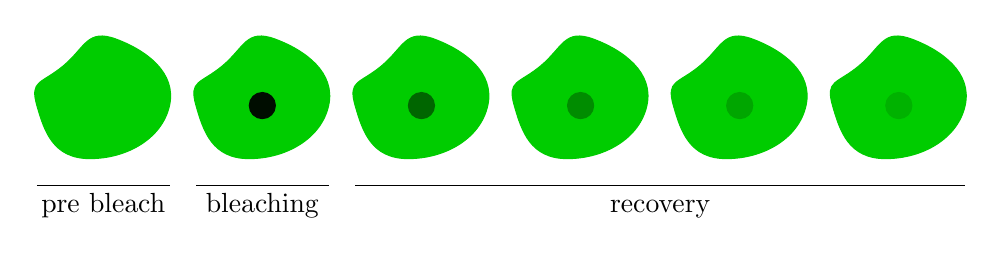
\begin{tikzpicture}[scale=\textwidth/7.2cm]
        \tikzset{drawandfill/.style={draw=#1,fill=#1}}

        %% I guess we should created a PGF shape for the cell and then
        %% we would use \path with cells at the nodes.  But oh boy, is
        %% that complicated?  It is definitely not worth having to pay
        %% university fees for another year so we just keep the cell
        %% size 1x1, and slide the x coordinates 1.2 for every cell.

        %% Draw the cells
        \foreach \offset in {0.0, 1.2, 2.4, 3.6, 4.8, 6.0} {%
          \draw[drawandfill=green!80!black]
          plot [smooth cycle, tension=1]
          coordinates {(\offset,0.5) (\offset+0.2,0.8) (\offset+0.6,1.0)
            (\offset+1.0,0.5) (\offset+0.4,0.1)}
          node at (\offset,0.0) {};
        }

        %% Draw the bleach spots
        \node at (1.7, 0.5) [circle, drawandfill=green!05!black] {};
        \node at (2.9, 0.5) [circle, drawandfill=green!40!black] {};
        \node at (4.1, 0.5) [circle, drawandfill=green!55!black] {};
        \node at (5.3, 0.5) [circle, drawandfill=green!65!black] {};
        \node at (6.5, 0.5) [circle, drawandfill=green!70!black] {};

        %% Write legend.  Specific text height and text depth values are
        %% required to align the text baselines.
        \tikzset{legend/.style={below,text height=1.5ex,text depth=.25ex}}
        \draw (0.0, -0.1) -- node[legend] {pre bleach} (1.0, -0.1);
        \draw (1.2, -0.1) -- node[legend] {bleaching}  (2.2, -0.1);
        \draw (2.4, -0.1) -- node[legend] {recovery}   (7.0, -0.1);

      \end{tikzpicture}

      %% Add some vertical space because the y axis of the plot below
      %% looks like it's pointing to the first cell.
      \bigskip

      %% Draw the plot of a recovery curve.
      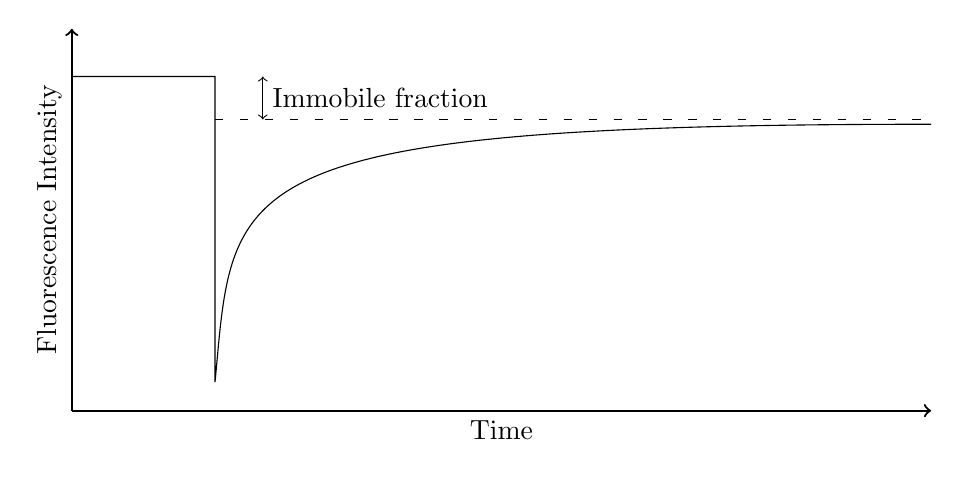
\begin{tikzpicture}[scale=\textwidth/10cm]
        \tikzset{axis/.style={thick,->}}
        \draw[axis] (0.5, 0.0)
                    -- node [below] {Time}
                    (9.5, 0.0);

        \draw[axis] (0.5, 0.0)
                    -- node[above, rotate=90] {Fluorescence Intensity}
                    (0.5, 4.0);

        \draw (0.5, 3.5)
              -- (2.0, 3.5)
              -- (2.0, 0.3)
              .. controls (2.2, 2.4) and (2.0, 3.0) .. (9.5, 3.0);

        \draw[<->] (2.5, 3.05)
                   -- node [right] {Immobile fraction}
                   (2.5, 3.5);

        \draw[loosely dashed] (2.0, 3.05) -- (9.5, 3.05);
      \end{tikzpicture}

      \captionIntro{Concept of a FRAP experiment}%
                   {The fluorescent proteins of a small region are
                    permanently bleached by a laser event. The
                    intensity in the region is measured so that the
                    plot shows the recovery of fluorescence in the
                    bleached area.  The recovery curve reflects the
                    diffusion and binding dynamics of the proteins
                    tagged with the fluorescent proteins.  The
                    fraction of fluorescence that does not recover is
                    the fraction of immobile proteins.}
      \label{fig:intro:frap-curve-example}
    \end{figure}

    In quantitative FRAP, data analysis involves fitting the recovery
    data to an idealized mathematical model.
    Many different models exist with different assumptions
    and dependencies on
    parameters \citep{mcnally-frap-2010}.
    Kinetic parameters are typically \kon{} and \koff{}, for
    binding and unbinding rate constants, and $D_{f}$ for the diffusion
    constant
    although a variety of additional parameters can be included in
    the design of FRAP models \citep{mcnally-frap-2010}.

    The compartment geometry must also be considered.  This includes
    deciding whether there are boundaries to the compartment or
    whether it is an infinite space.  A simplification of the
    compartment from a three dimensional volume to a two dimensional
    area can be applied.

    The bleaching event is a source of considerable variability.
    The time interval between the bleaching and the acquisition of the
    first image is a window where recovery of a mobile fraction might
    happen.  Likewise, the bleaching event is not
    instantaneous and will occur while molecules are exchanging.
    The shape of the bleached area is a parameter and the
    profile of the laser beam will have an effect that can be modelled
    as either a gaussian or a flat-top distribution.

    Diffusion rates may be fixed, fitted, or assumed to be instantaneous.
    A single diffusion rate may be assumed for the whole
    compartment, or non-homogeneous regions in the compartment
    can have different diffusion rates.

    Finally, if binding to a complex is considered, a
    plethora of additional potential parameters are introduced.  Multiple
    binding states may be present when binding reactions occur in a
    series of steps involving multiple proteins, and the distribution of
    the binding sites may be not equal throughout the compartment.

    While all these many features may appear
    as parameters in the mathematical model for
    fitting to a FRAP curve, they also affect how the experiment is performed.

    FRAP has a number of implicit assumptions which are applicable
    for most biological situations.
    Firstly, the biological system is assumed to have
    reached equilibrium and the equilibrium
    is maintained throughout the experiment.
    This means the kinetic parameters
    must remain constant throughout the experiment.
    Secondly, the distribution of the tagged protein mimics the endogenous
    protein.
    And finally, the binding sites
    should be part of a large, relatively immobile
    complex on the time and length scale of the recovery.
    These assumptions become difficult to maintain as the experiment
    times increases for slow moving molecules.

\section{Bioinformatics}

  With the advent of genomic and transcriptomic
  sequencing, and with the development of super resolution microscopy,
  a biology laboratory can easily generate several gigabytes of data
  in a single set of experiments.
  Even laboratories that lack access to the required equipment can
  easily access these amounts of data in public repositories.
  The analysis of this data is becoming a bottleneck for research
  advances \citep{marx2013biology-big-data} so the development of
  tools to handle large datasets is a race against the technology that
  generates it \citep{delisi1988computers-molecular-biology}.
  This has led to the rise of a new field of science,
  bioinformatics, for the research of software tools for the
  acquisition, storage, and analysis of biological data.

  In this context, computers have become an
  essential tool in all areas of biological research
  \citep{wren2016bioinformatics}.
  A researcher will use a computer on a daily
  basis as an enabling device for their research.
  DNA and protein sequences are computer files to be analysed by specialised
  software.  Cloning strategies are planned with the help of software.
  Sequences are searched for in large databases and compared against other
  sequences for similarities.
  Likewise, the structure of biomolecules is predicted by software and
  visualised in 3D in a computer.  Microscopes are controlled by
  computers, such that the images acquired by electronic cameras mean
  eyepieces are now optional.  Even
  literature review is performed in a computer with new publications
  revealed by searching in online databases rather than
  by browsing issues in libraries.  Software is
  thus essential for science and is a daily tool of the scientist.

  However, despite the ubiquity of software in biology, laboratories
  struggle to find appropriate researchers capable of handling the data
  \citep{lakhani2013prize}.  Just like the development software of tools has
  been lagging behind data generation
  since 1990s, so has the training of biologists
  for bioinformatics \citep{altman1998curriculum}.
  Nevertheless, the challenges for career progression that
  bioinformaticians face in academia provides little incentive for
  change \citep{wren2016bioinformatics}.

  \subsection{Free Software and Scientific Advances}

  Scientific discoveries are almost always incremental on previous work.
  This is true not only for new theories but also
  for methods, since new techniques are usually generated by
  a constant iteration of improvements.  Software used by
  scientists is also a tool and should allow for such a
  series of iterative improvements.

  Outside of academia, lack of access to the source code of the software
  is also an issue.  The problem has led to
  multiple organisations being formed to promote the ability of users
  to modify the software they use so it works for their own
  purposes.

  Two of the main proponents of this philosophy
  are the Free Software Foundation and the
  Open Source Initiative.  The Free Software Foundation defines free
  software as providing the four basic freedoms: Freedom to run a
  program for any purpose, freedom to study the source code of the program,
  freedom to distribute the program,
  and freedom to distribute modified versions of the program
  \citep{fsf-what-is-free-software}.
  In fact,
  the free software movement began in academia itself, by
  Richard Stallman at the MIT Artifical Intelligence lab.  This was
  triggered by a series of events caused by non-free software, when
  an AI lab spin-off made its software non-free, and the lab mainframe
  was replaced with another that ran on non-free software
  \citep{stallman-essays}.
  %% Stallman quit the job at MIT to develop GNU but the AI lab let
  %% him stay around for the work anyway.

  \subsection{Free Software Projects in Academia}
  This growing openness and sharing of code to enable incremental
  development of scientific software is becoming recognised as an
  important driver of progress in highly data driven research fields.

  Despite the lack of computational details in the data analysis,
  free software is widely used in biological research,
  and multiple projects exist
  for enabling data analysis in molecular cell biology.
  This demonstrates that free software does enable research.
  For example, BioPerl is a large project for the handling of biological
  data in the Perl programming language and was heavily involved in
  facilitating the sequencing of the human genome \citep{bioperl}.
  Following its success, similar projects have been
  created for the Python and Java languages,
  Biopython \citep{biopython} and BioJava \citep{biojava}
  respectively.
  Many programming languages used by bioscience researchers are themselves
  free software, including R \citep{R-manual}, GNU
  Octave \citep{octave}, and Julia \citep{julia}.
  Similarly, interactive applications have also been
  created for a wide range of purposes such as
  ImageJ for image analysis \citep{imagej1}, GBrowse for
  annotation and browsing genomic data \citep{gbrowse},
  and OMERO for data storage \citep{omero}.

  \subsection{Meta-research}

  The lack of access to sufficient code in
  publications not only delays research by
  obliging investigators to redo the work of others to build on it, but also
  increases the difficulty of validating research
  by making published experiments unable to be reproduced.
  For example, for a survey of 18 published microarray gene-expression
  studies, it took a team of data analysts an average of half a week
  to replicate a single figure or table, with some figures taking more
  than one week.  Only two of the 18 figures were ``reproducible in
  principle'', that is, with differences that were considered to be minor
  \citep{ioannidis2009repeatability}.
  Difficulty with reproducibility
  does not imply that results have been fabricated.
  The main problem identified was the lack of availability
  of data, and the second was the lack of detail on how to perform the
  analysis.

  This reproducibility gap has become a growing issue in recent years and led to
  the creation of the new field of meta-research, for the investigation of the
  research practice \citep{ioannidis2015meta, collins2014researching}.

  With computers being central to analysis, one would
  expect that analysis could be readily shared in the form of source code.
  However, that is not the case.  Publications favour a natural
  language description of the analysis which lacks the level of
  detail that would allow others to repeat or improve on
  work \citep{ince2012case}.
  An indirect cause of this anomaly is that
  scientists share their work through print-centred articles
  and books that are far from ideal media for complicated source
  code or procedural instructions.
  There is a growing
  interest within the scientific community to improve the situation
  and journals have been changing their policies to promote sharing of
  source code \citep{nature-code-share-editorial, gmd-editorial-2013,
    stodden2013toward}.

\section{Aims and Objectives}

  Histones organise the fundamental nucleosomal level of chromatin and
  although the static structure of  nucleosomes is
  known, their dynamic properties are poorly understood.  Current
  models of nucleosome dynamics are largely based on \textit{in vitro}
  experiments and observations in unicellular yeast
  which are largely composed of euchromatin.  We wished to apply FRAP to test
  models of nucleosome dynamics in human cells and their dependence on
  amino acid variations in core histones.

  While canonical core histones are usually referred to as single
  proteins by their type H2A, H2B,
  H3, or H4 only, they actually comprise a family of isoforms whose
  sequence differences are rarely recognised.
  We required a catalogue of the human histones to understand this
  sequence variation as a basis for the FRAP investigation
  but the last version of such an inventory had been performed in
  2002, before the finalisation of the human genome \citep{Marzluff02}.
  Therefore, we assembled an up to
  date catalogue of all human core histones presented in
  \Cref{ch:histone-catalogue}.  Recognising the inevitable
  changes to such catalogues over time, we automated its creation so that a
  constantly up to date version could be generated with little effort.

  As a first attempt to apply FRAP as a tool for measuring the effect of
  histone sequences on mobility in cell nuclei we chose to investigate
  the stability of core histone SIN mutations.
  We faced complications with
  long time frame FRAP measurements.  In \Cref{ch:kill-frap} we detail our
  step-wise approach to solving these issues.

  Through these studies, we developed many software components and
  strove to improve existing tools that would be available to all
  researchers.  In \Cref{ch:software} we describe the multiple tools
  created and improved, all of which have been released under a free
  software licence.

  Inspired by the principles of reproducible research, all the source
  for this thesis is also available with a build system to automate its
  construction from the raw data.  This thesis is itself part of our
  broader effort to investigate
  the application of software development tools for the maintenance of
  reproducible research.
